In order to compare the inflatable decelerator concepts in terms of mass, the total decelerator structural mass as yielded by the methods outlined in section \ref{sec:strucmeth} is computed for each of the four inflatable concepts. Due to the limited applicability of each of the methods used, a necessity is the use of multiple methods: the method by Samareh \cite{Samareh2011} for the mass estimation of stacked toroid, tension cone and trailing \gls{iad} concepts; the method by Anderson \cite{Anderson1969} for the mass estimation of the isotensoid.

\begin{figure}[H]
\hspace{-14mm}
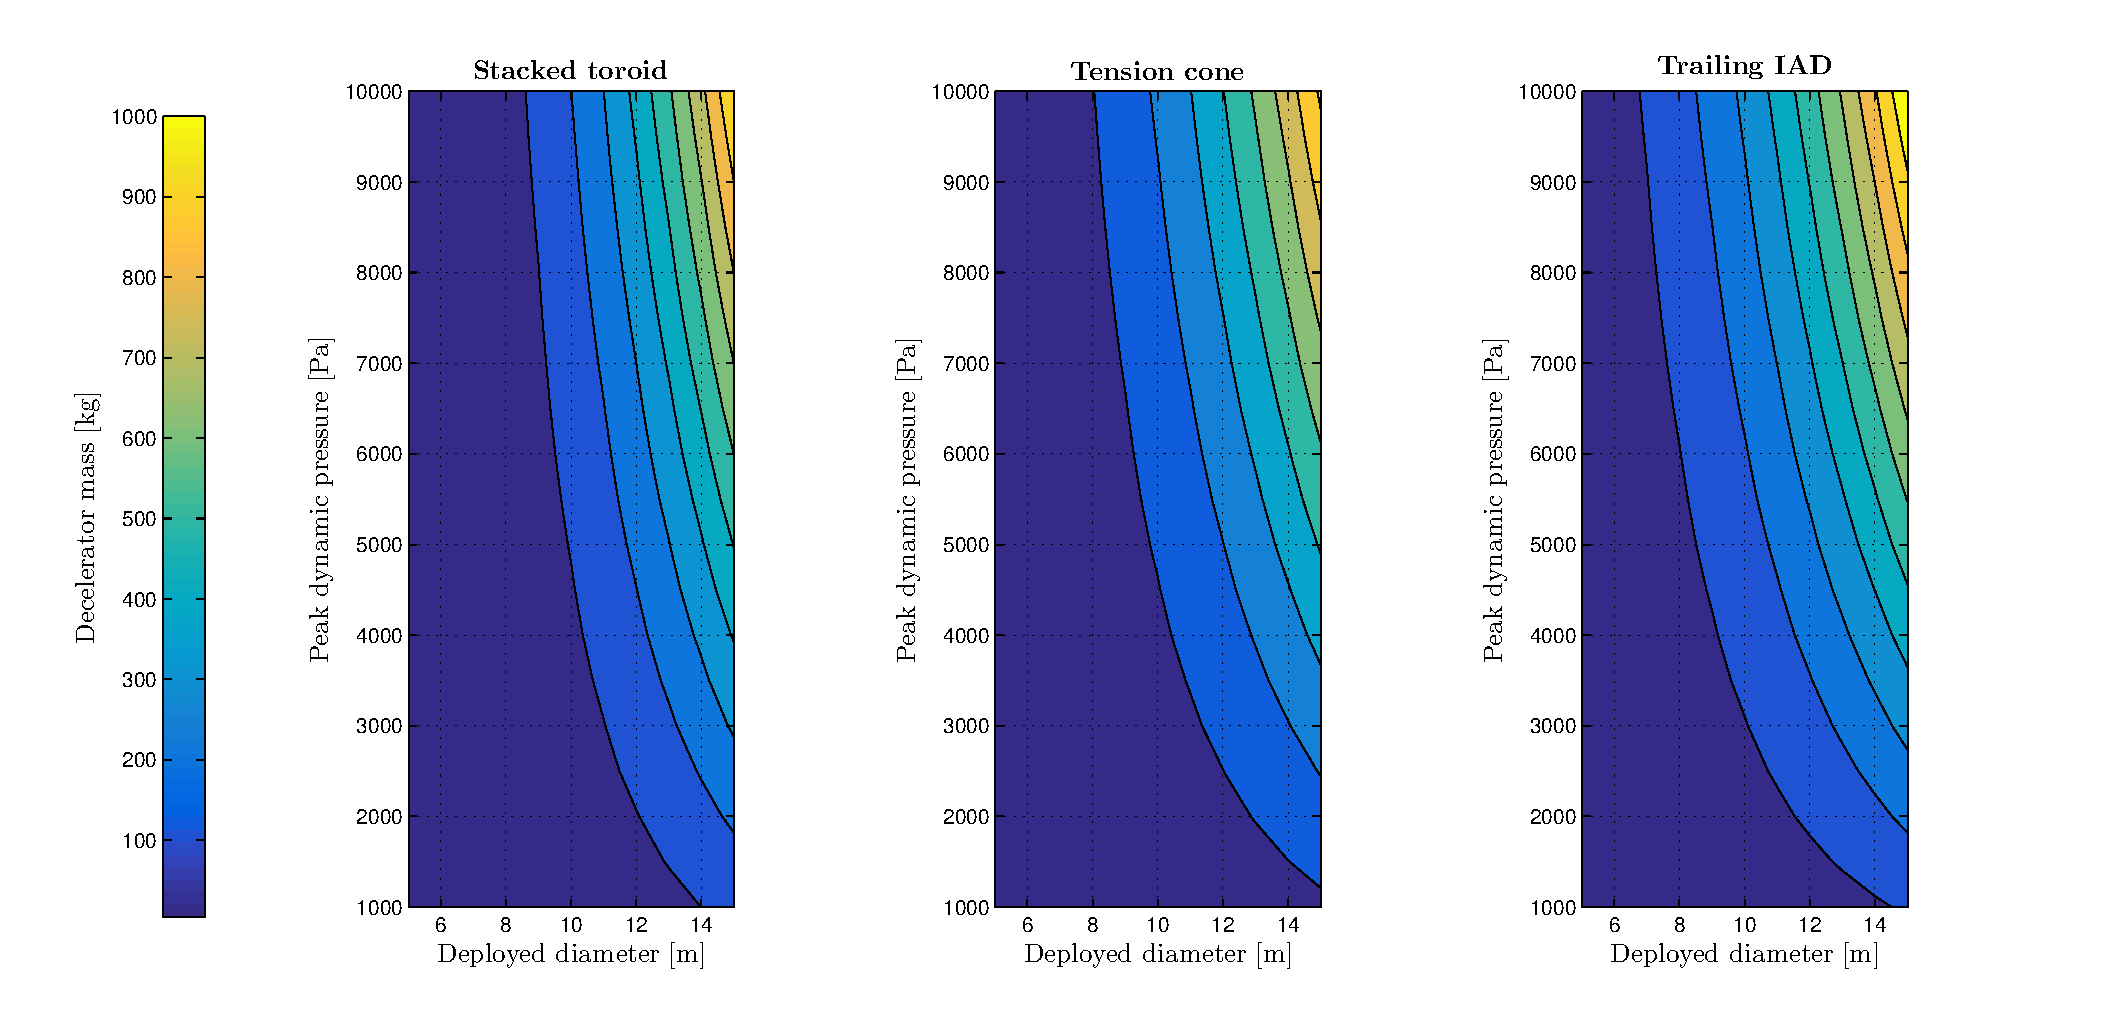
\includegraphics[width = 1.2\textwidth]{Figure/mass_dia_qmax.eps}
\caption{\acrlong{dot} for mission duration}
\label{fig:mass_dia_qmax}
\end{figure}

\begin{figure}[H]
\centering
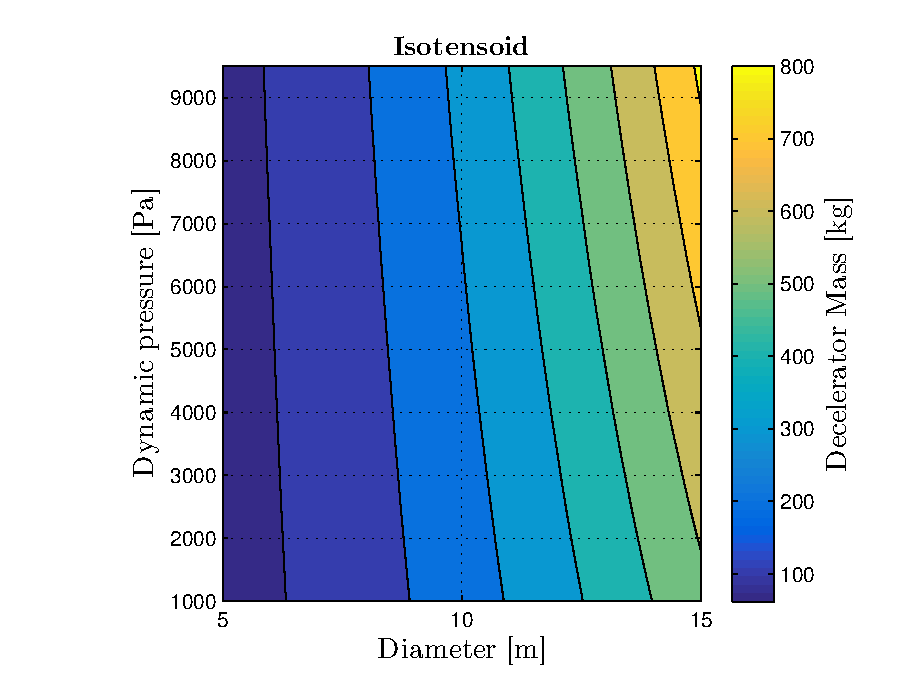
\includegraphics[width = 0.55\textwidth]{Figure/ISO_comp.eps}
\caption{\acrlong{dot} for mission duration}
\label{fig:ISO_comp}
\end{figure}

%Fig.\ref{fig:mass_dia} gives the total structural decelerator mass Figure \ref{fig:mass_dia} was made with a peak dynamic pressure of $\gls{sym:q}=3000$ [$Pa$], a drag coefficient $\gls{sym:CD}=1.5$ [$-$] and Vectran for inflatable decelerator material.

Figures \ref{fig:mass_dia_qmax} and \ref{fig:ISO_comp} show the total structural decelerator mass for the stacked toroid, tension cone, trailing ballute and isotensoid configurations, for a drag coefficient of 1.5 [-]. An increase or decrease in drag coefficient has, qualitatively, the same effect as an increase or decrease in dynamic pressure respectively. Total mass has been plotted as a function of peak dynamic pressure on one hand to display its dependence on loading conditions, as the peak dynamic pressure can be treated as a surrogate for the maximum structural loads, and as a function of deployed diameter on the other hand, since this is the primary design parameter used in the orbital analysis. As both factors are held variable before concept selection after trade-off, concepts are evaluated for their mass performance over the ranges considered. Peak dynamic pressures from 1000 to 10000 [Pa] are deemed representative, based on reference missions and the orbital analysis tool; diameter is constrained to 12 [m] but evaluated up to 15 [m] for the sake of completeness. 

From Figures \ref{fig:mass_dia_qmax} and \ref{fig:ISO_comp} it can be concluded that

Fig.\ref{fig:mass_dia} serves to show how each different configurations mass scales with varying deployed diameter. It can be noted that the isotensoid configuration has a relatively, compared to the other inflatable concepts, high mass at the base diameter of five meters. This can be attributed to the fact that the isotensoid configuration features no deployed diameter. Different from the other inflatable concepts described by the model of Samareh in which the undeployed diameter has direct links the the mass of for example the gas system. The isotensoid configuration, among featuring no pressurised gas inflation system but rather ram-air, has no such diameter defined. The isotensoid is a single all compassing inflatable covering the whole payload. 

Although plotted for set values of the drag coefficient, peak dynamic pressure and further configuration parameters important remarks with respect to the isotensoid design can already be made. If looking solely of the structural mass performance of the decelerator concepts a isotensoid configuration is the least preferable. This is further reinforced by the sensitivity analysis of section \ref{sec:strucsens} in which configuration sensitivity is further considered. 

\begin{figure}[H]
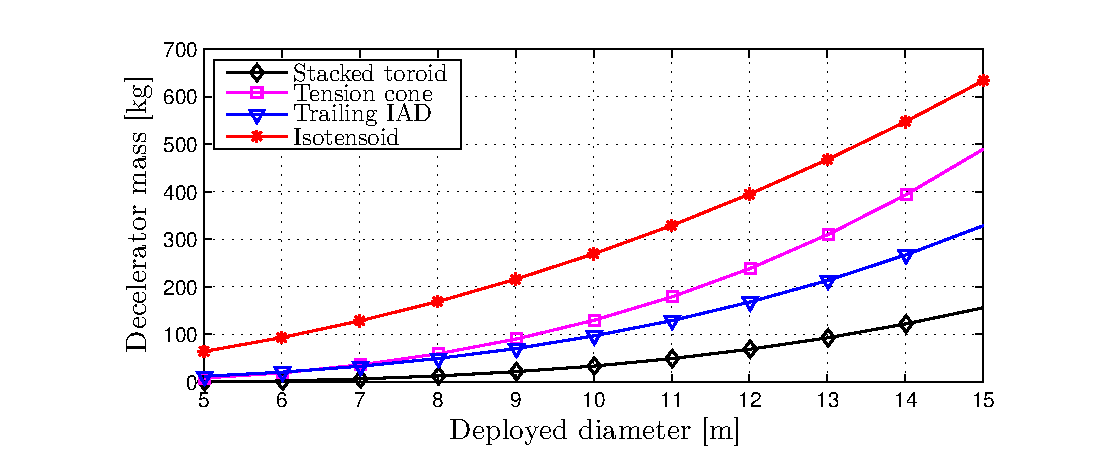
\includegraphics[width = 1.0\textwidth]{Figure/mass_dia.eps}
\caption{Decelerator mass versus deployed diameter for all the inflatable configurations}
\label{fig:mass_dia}
\end{figure}
